\pdfobjcompresslevel=0
\pdfminorversion=4
\documentclass{beamer}
\usepackage{multimedia}
%\usepackage[pdftex]{graphicx}
%\usepackage{graphviz}
\usepackage{graphviz}
%===Pick Theme===
\usetheme{Warsaw}
\usecolortheme{beaver}
\useoutertheme{infolines}
\useinnertheme{circles}

%===Customize Theme=== %
\setbeamercolor{item}{fg=darkred}
\setbeamertemplate{itemize subitem}{$\circ$}
\setbeamercolor*{block title}{fg=white, bg=darkred}
\setbeamercolor*{block body}{bg=lightgray}

%===Set the covered style=== %
\setbeamercovered{transparent}
%===Set the bib reference key style=== %
\setbeamertemplate{bibliography item}[text]
%===Disable navigation bar=== %
\setbeamertemplate{navigation symbols}{}%remove navigation symbols

\usepackage{minted}
\setminted[python]{bgcolor=bg,fontsize=\scriptsize,linenos,xleftmargin=8pt}
\setmintedinline[python]{bgcolor=bg,fontsize=\scriptsize}
\setmintedinline[bash]{bgcolor=bg,fontsize=\scriptsize}
\setminted[xml]{bgcolor=bg,fontsize=\scriptsize,linenos,xleftmargin=8pt}
\setmintedinline[xml]{bgcolor=bg,fontsize=\scriptsize}
\newcommand{\pyinline}[1]{\mintinline{python}{#1}}
\newcommand{\bashinline}[1]{\mintinline{bash}{#1}}
%===Logos=== %

%\usepackage{pgf}
%\logo{\pgfputat{\pgfxy(-1,7)}{\pgfbox[center,base]{
\includegraphics[height=0.5in]{fig/duckietown_logo}}}}

\logo{
\includegraphics[height=0.5in]{fig/duckietown_logo}}
\titlegraphic{ %
\centering

\includegraphics[height=1.8in]{fig/duckietown_logo}%\hspace{2ex}
%\raisebox{-0.75in}{
\includegraphics[height=1.5in]{fig/indigoigloo_600.png}}
} %


\author[Shih-Yuan Liu]{Shih-Yuan Liu}
\title[ROS in Duckietown]{Robot Operating System (ROS) in Duckietown}
\institute[Duckietown MIT]{Duckietown, MIT}
\date[Feb. 16th, 2016]{February 16th 2016}

\begin{document}
\definecolor{bg}{rgb}{0.95,0.95,0.95}

\begin{frame}[plain,label=titlepage,noframenumbering] %[plain,noframenumbering] will not show the header and footer
	\titlepage
\end{frame}

\begin{frame}[label=overview]{Overview}
	\tableofcontents
	%\tableofcontents[sectionstyle=show/shaded,subsectionstyle=show/shaded/shaded]
\end{frame}


\section{Introduction}

\begin{frame}{What is ROS?}
\begin{columns}
	\begin{column}{0.55\textwidth}
		Robotics Operating System (ROS) is an \alert{open-source}, \alert{meta-operating system} for your \alert{robot}:
		\begin{itemize}
			\item Hardware abstraction and low-level device control
			\item Message-passing between processes
			\item Package and build management system
			\item Data visualization, logging, and analysis
		\end{itemize}
	\end{column}
	\begin{column}{0.45\textwidth}
		\centering
		
\includegraphics[width=\textwidth]{fig/indigoigloo_600.png}
	\end{column}
\end{columns}
\end{frame}

\begin{frame}{Why ROS?}
\begin{columns}
	\begin{column}{0.55\textwidth}
		\begin{itemize}
			\item Open-source
			\item Well documented
			\item \alert{\texttt{python}} for accessibility and \alert{\texttt{C++}} for performance 
			\item Native to \alert{Ubuntu}, available to other OS via virtual machines
			\item Active community with \alert{3000+} packages
		\end{itemize}
	\end{column}
	\begin{column}{0.45\textwidth}
		\centering
		
\includegraphics[width=\textwidth]{fig/indigoigloo_600.png}
	\end{column}
\end{columns}
\onslide<2>{
\begin{block}{Is there a ROS package for $x$? Can ROS do $y$?}
	Most likely YES!
\end{block}}

\end{frame}

\section{ROS Concept Overview}
\begin{frame}[label=overview]{Overview}
%	\tableofcontents
	\tableofcontents[sectionstyle=show/shaded,subsectionstyle=show/shaded/shaded]
\end{frame}

\subsection{Nodes and Topics}
\begin{frame}{Nodes and Topics}
	\begin{columns}[c]
		\begin{column}{0.6\textwidth}
			\begin{itemize}
				\item Nodes:
					\begin{itemize}
					\item Executables (\texttt{python} or \texttt{C++})
					\item Each node is a process
					\item Publishes/Subscribes to Topics
					\end{itemize}
				\item Topics:
					\begin{itemize}
					\item Passes information between nodes
					\item Topic type defined by messages
					\item Support many-to-many communication
					\end{itemize}
			\end{itemize}
		\end{column}
		\begin{column}{0.4\textwidth}
			% \centering
			\includedot[width=\textwidth,height=\textheight,keepaspectratio]{dot/node_and_topic}
		\end{column}
	\end{columns}
\end{frame}

\begin{frame}{Publisher Node Example}
	\inputminted{python}{snippet/publisher_node.py}
\end{frame}

\begin{frame}{Subscriber Node Example}
	\inputminted{python}{snippet/subscriber_node.py}
\end{frame}

\begin{frame}{Related Tools and Demo}
	\begin{columns}
		\begin{column}{0.3\textwidth}
			\begin{itemize}
				\item \mintinline{bash}{rosrun}
				\item \mintinline{bash}{rosnode list}
				\item \mintinline{bash}{rosnode info}
				\item \mintinline{bash}{rostopic info}
				\item \mintinline{bash}{rostopic list}
				\item \mintinline{bash}{rqt_graph}
			\end{itemize}
		\end{column}
		\begin{column}{0.7\textwidth}
			\centering
			Live demo here.
		\end{column}
	\end{columns}
\end{frame}

\subsection{Packages}
\begin{frame}{Packages}
\begin{columns}
	\begin{column}{0.6\textwidth}
		\begin{itemize}
			\item Packages are organization tools for:
			\begin{itemize}
				\item Functionality
				\item Build and runtime dependencies
				\item Namespaces
			\end{itemize}
			\item Key Files
				\begin{itemize}
					\item CMakeLists.txt
					\item package.xml
					\item setup.py
				\end{itemize}
			\item Tools
				\begin{itemize}
					\item \mintinline{bash}{roscd}
					\item \mintinline{bash}{rospack profile}
					\item \mintinline{bash}{rospack depends}
				\end{itemize}
		\end{itemize}
	\end{column}
	\begin{column}{0.4\textwidth}
		\centering
		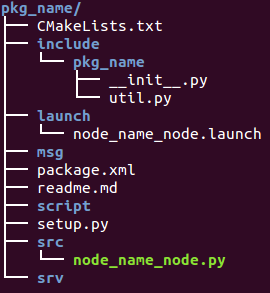
\includegraphics[width=\textwidth]{fig/pkg_tree.png}
	\end{column}
\end{columns}
\end{frame}

\begin{frame}{ROS Master}
	\begin{columns}[T]
		\begin{column}{0.6\textwidth}
			\begin{itemize}
			\item Handles communication between nodes
			\item Connects publisher and subscriber
			\item Traffic does \alert{not} go through the master once connected
			\item TCP/IP connection
			\item \bashinline{roscore}
			\end{itemize}
		\end{column}
		\begin{column}{0.4\textwidth}
			\centering
			\includegraphics[width=\textwidth]{fig/tele_operator.jpg}
		\end{column}
	\end{columns}
	\only<1>{\includedot[width=\textwidth,height=\textheight,keepaspectratio]{dot/master_1}}
	\only<2>{\includedot[width=\textwidth,height=\textheight,keepaspectratio]{dot/master_2}}
	\only<3>{\includedot[width=\textwidth,height=\textheight,keepaspectratio]{dot/master_3}}
	\only<4>{\includedot[width=\textwidth,height=\textheight,keepaspectratio]{dot/master_4}}
	\only<5>{\includedot[width=\textwidth,height=\textheight,keepaspectratio]{dot/master_5}}
\end{frame}


\begin{frame}{Parameters}
	\begin{columns}
		\begin{column}{0.6\textwidth}
			\begin{itemize}
				\item Nodes can set/get parameters to/from the parameter server
				\item Parameters can be changed during run time
				\item Parameters can be load/dump to yaml files 
				\item Provides simple parameterization of nodes
				\item Tools:
					\begin{itemize}
						\item \bashinline{rosparam list}
						\item \bashinline{rosparam get/set}
						\item \bashinline{rosparam load/dump}
					\end{itemize}
			\end{itemize}
		\end{column}
	\begin{column}{0.4\textwidth}
		\centering
		TODO: Parameter example of camera.launch and joystick.launch
		%\includegraphics[width=\textwidth]{}
		\end{column}
	\end{columns}
\end{frame}

\begin{frame}{Launch Files}
	\begin{columns}
		\begin{column}{0.6\textwidth}
			\begin{itemize}
				\item ROS specific scripts as XML
				\item Capabilities:
					\begin{itemize}
						\item Launch nodes
						\item Set node names
						\item Set/Load parameters
						\item Remap topics
						\item Specify machines
						\item Configuration at launch time through \bashinline{<arg>}
					\end{itemize}
				\item Tools:
					\begin{itemize}
						\item \bashinline{roslaunch --args}
						\item \bashinline{roslaunch --find}
						\item \bashinline{roslaunch --ros-args}
					\end{itemize}
				\item In Duckietown:
					\begin{itemize}
						\item Each node has one elemental launch file
						\item Documents the I/O of a node
						\item Standard interfaces through \bashinline{<arg>}
					\end{itemize}
			\end{itemize}
		\end{column}
	\begin{column}{0.4\textwidth}
		\centering
		TODO: example using camera.launch and joystick.launch
		DEMO: command line argument --args --ros-arg --find etc
		%\includegraphics[width=\textwidth]{}
		\end{column}
	\end{columns}
\end{frame}

\begin{frame}{Services}
	TODO
\end{frame}

\section{Best Practices in Duckietown}
\begin{frame}{Duckietown ROS guidelines}
	\begin{columns}
		\begin{column}{0.6\textwidth}
			\begin{itemize}
				\item TODO
			\end{itemize}
		\end{column}
		\begin{column}{0.4\textwidth}
			\centering
			%\includegraphics[width=\textwidth]{}
		\end{column}
	\end{columns}
\end{frame}

\section{ROS Architecture in Duckeitown}

\begin{frame}{Duckietown ROS Diagram}
TODO: whole diagram. Meant to be overwhelming. Then we break it down into modules
\end{frame}


\begin{frame}{Joystick (Remote Control)}
	\begin{columns}
		\begin{column}{0.4\textwidth}
			\begin{itemize}
				\item \bashinline{joy}
				\item \bashinline{joy_mapper_node}
				\item \bashinline{wheels_trimmer_node}
				\item \bashinline{wheels_driver_node}
			\end{itemize}
		\end{column}
		\begin{column}{0.6\textwidth}
			\centering \includedot[width=\textwidth,height=\textheight,keepaspectratio]{dot/joystick}
		\end{column}
	\end{columns}
\end{frame}

\begin{frame}{Camera (Data Processing)}
	\begin{columns}
		\begin{column}{0.42\textwidth}
			\begin{itemize}
				\item \bashinline{camera_node}
				\item \bashinline{decoder_node}
				\item \bashinline{cam_info_reader_node}
				\item \bashinline{intrinsic_calibration_file}
			\end{itemize}
		\end{column}
		\begin{column}{0.58\textwidth}
			\centering
			\includedot[width=\textwidth,height=\textheight,keepaspectratio]{dot/camera}
		\end{column}
	\end{columns}
\end{frame}

\begin{frame}{Lane Filter (Filtering)}
	\begin{columns}
		\begin{column}{0.42\textwidth}
			\begin{itemize}
				\item \bashinline{line_detector_node}
				\item \bashinline{ground_projection_node}
				\item \bashinline{lane_filter_node}
				\item \bashinline{extrinsic_calibration_file}
			\end{itemize}
		\end{column}
		\begin{column}{0.58\textwidth}
			\centering
			\includedot[width=\textwidth,height=\textheight,keepaspectratio]{dot/lane_filter}
		\end{column}
	\end{columns}
\end{frame}

\begin{frame}{Lane Control (Vision-Based Control)}
	\begin{columns}
		\begin{column}{0.6\textwidth}
			\begin{itemize}
				\item 
			\end{itemize}
		\end{column}
		\begin{column}{0.4\textwidth}
			\centering
			TODO: add figure
		\end{column}
	\end{columns}
\end{frame}

\begin{frame}{Planning}
	\begin{columns}
		\begin{column}{0.6\textwidth}
			\begin{itemize}
				\item 
			\end{itemize}
		\end{column}
		\begin{column}{0.4\textwidth}
			\centering
			%\includegraphics[width=\textwidth]{}
		\end{column}
	\end{columns}
\end{frame}

\begin{frame}{Localization}
	\begin{columns}
		\begin{column}{0.6\textwidth}
			\begin{itemize}
				\item 
			\end{itemize}
		\end{column}
		\begin{column}{0.4\textwidth}
			\centering
			%\includegraphics[width=\textwidth]{}
		\end{column}
	\end{columns}
\end{frame}

\begin{frame}{Coordination}
	\begin{columns}
		\begin{column}{0.6\textwidth}
			\begin{itemize}
				\item 
			\end{itemize}
		\end{column}
		\begin{column}{0.4\textwidth}
			\centering
			%\includegraphics[width=\textwidth]{}
		\end{column}
	\end{columns}
\end{frame}

% \begin{frame}{Duckietown ROS guidelines}
% \end{frame}

\begin{frame}{Resources}
  \begin{columns}
	\begin{column}{0.6\textwidth}
	  \begin{itemize}
		\item TODO: links to ROS tutorial and wiki
	  \end{itemize}
	\end{column}
  \begin{column}{0.4\textwidth}
		\centering
		%\includegraphics[width=\textwidth]{}
		% \digraph[scale=0.5]{abc}{a->b->c;}
	\end{column}
  \end{columns}
\end{frame}

% \begin{frame}{Duckietown ROS Diagram}
%	\digraph[scale=0.2]{aaa}{\input{dot/duckietown}}
	% \includedot[scale=0.8]{dot/test}
% \end{frame}

%\begin{frame}{Snippet}
%	\begin{itemize}[<+->]
%		\item Hey
%		\inputminted{python}{snippet/test.py}
%		\item Ho \mintinline{python}{import numpy as np}
%	\end{itemize}
%\end{frame}

\end{document}